%%%%%%%%%%%%%%%%%%%%%%%%%%%%%%%%%%%%%%%%%%%%%%%%%%%%%%%%%%%%%%%%%%%%%%%%%
%%%%%%%%%%%%%%%%%%%%%%%%%%%%%%%%%%%%%%%%%%%%%%%%%%%%%%% Art des Dokuments
%%%%%%%%%%%%%%%%%%%%%%%%%%%%%%%%%%%%%%%%%%%%%%%%%%%%%%%%%%%%%%%%%%%%%%%%%
\documentclass[oneside,a4paper]{article}
%\documentclass[12pt,a4paper,twoside,ngerman]{book}
%\documentclass[12pt,oneside,a4paper]{scrartcl}
%\documentclass[10pt, a4paper, landscape]{letter}
%\documentclass[11pt,a4paper]{article}
%\documentclass[12pt,a4paper]{dissertation}
%\documentclass[t]{beamer}

%%%%%%%%%%%%%%%%%%%%%%%%%%%%%%%%%%%%%%%%%%%%%%%%%%%%%%%%%%%%%%%%%%%%%%%%%
%%%%%%%%%%%%%%%%%%%%%%%%%%%%%%%%%%%%%%%%%%%%%%%%%%%%%%%%%%%%%%%%%%% Fonts
%%%%%%%%%%%%%%%%%%%%%%%%%%%%%%%%%%%%%%%%%%%%%%%%%%%%%%%%%%%%%%%%%%%%%%%%%
\usepackage[utf8]{inputenc} % Einlesen von Umlauten 
\usepackage[T1]{fontenc} % Darstellung von Umlauten
\usepackage[ngerman]{babel} % Silbentrennung
\newcommand{\hide}[1]{  }

\usepackage{hyperref}  % Referenzen
\usepackage{natbib} 	% Zitieren
\usepackage{ifthen} %% Fallunterscheidungen
	%\ifthenelse{\equal{#1}{\empty}}{#then}{#else}
	%\IfFileExists{file}{then-code}{else-code}
	%\InputIfFileExists{file}{then-code}{else-code}


%\usepackage{lmodern}
%\usepackage{concrete}% fancy fonts
%\usepackage{color} % for fancy section font and color
%\allsectionsfont{\color{section_color}\sffamily\selectfont}
%\usepackage{xcolor} % colour tricks ;)
%\definecolor{section_color}{rgb}{0.35,0.0,0}
%\usepackage{textcomp} % verschiedene Sonderzeichen, z.b. Euro
%%%%%%%%%%%%%%%%%%%%%%%%%%%%%%%%%%%%%%%%%%%%%%%%%%%%%%%%%%%%%%%%%%%%%%%%%
%%%%%%%%%%%%%%%%%%%%%%%%%%%%%%%%%%%%%%%%%%%%%%%%%%%%%% Seitenformatierung
%%%%%%%%%%%%%%%%%%%%%%%%%%%%%%%%%%%%%%%%%%%%%%%%%%%%%%%%%%%%%%%%%%%%%%%%%
%\usepackage{layout}  % \layout
%\usepackage{geometry} % page layout options
%\usepackage[a4paper]{typearea} %\a6paper: DIN A6 (1051mm x 1481mm) 
%\geometry{  
%			head = 5mm, foot = 5mm, 
%			landscape,
%			papersize={74mm,52mm},
%			text={60mm, 35mm},
%			left=3cm,right=3cm,top=2cm,bottom=3cm,
%			includeheadfoot
%}
%\usepackage{fancyhdr}
%\fancyhead[LCR]{bsp} 
%\fancyfoot[LCR]{bsp}
%\renewcommand{\headrulewidth}{0.5pt}
%\renewcommand{\footrulewidth}{0.5pt}
%\fancyhf{} % clear all header and footer fields
%\setlength{\textwidth}{15.5cm}
%\setlength{\textheight}{23cm}
%\setlength{\topmargin}{0cm}
%\setlength{\oddsidemargin}{0.5cm}
%\setlength{\evensidemargin}{0cm}
%\setlength{\parskip}{1ex}
%\setlength{\parindent}{0cm}
%\setcounter{tocdepth}{4}
%\setcounter{secnumdepth}{4}
%\headheight16.0pt
%%%%%%%%%%%%%%%%%%%%%%%%%%%%%%%%%%%%%%%%%%%%%%%%%%%%%%%%%%%%%%%%%%%%%%%%%
%%%%%%%%%%%%%%%%%%%%%%%%%%%%%%%%%%%%%%%%%%%%%%%%%%%%%%%% Textformatierung
%%%%%%%%%%%%%%%%%%%%%%%%%%%%%%%%%%%%%%%%%%%%%%%%%%%%%%%%%%%%%%%%%%%%%%%%%
%\usepackage{blindtext} % \blindtext
%\usepackage{indentfirst} % indent
%\setlength{\parskip}{0.3cm}
%\setlength{\parindent}{5pt}
% \renewcommand{\baselinestretch}{1.1}
%\marginparwidth = 10pt
%\footskip0mm
%\hoffset-10mm
%\voffset-5pt
%\normalheading % Überschriftengröße auf zur Schriftgröße angepaßt
%\usepackage{microtype} % für Blocksatz \flushright \flushleft
%\clubpenalty = 10000 % Disable single lines at the start of a paragraph (Schusterjungen)
%\widowpenalty = 10000 \displaywidowpenalty = 10000 % Disable single lines at the end of a paragraph (Hurenkinder)
\usepackage{multicol} % Mehrere Spalten \begin{multicols}{2}  \end{multicols}
%\usepackage{multirow}  % In Tabelle Zeilen zusammenfassen
%\usepackage{multicolumn} % In Tabelle Spalten zusammenfassen
%\usepackage{pdflscape}% landscape environment
%\usepackage[square,numbers]{natbib}% fuer Zitate
%\usepackage[babel,german=quotes]{csquotes}% fuer Zitate
%\newcommand{\Banach}{\textsc{Banach}} % Kapitaelchen
%\usepackage{longtable} % Mehrseitige Tabellen
%\usepackage{tabularx} % Tabellen mit fester Gesamtbreite und variablen Spalten

\hide{ 
\renewcommand\cite[2][]{ \ifthenelse{\equal{#1}{\empty}}
	{(\citeauthor{#2} \citeyear{#2})}
	{(\citeauthor{#2} \citeyear{#2}, S. #1)}
}
\newcommand\fcite[2][]{\ifthenelse{\equal{#1}{\empty}}
	{\footnote{\citeauthor{#2} \citeyear{#2}}.}
	{\footnote{\citeauthor{#2} \citeyear{#2}, S. #1}.}
}
}
%%%%%%%%%%%%%%%%%%%%%%%%%%%%%%%%%%%%%%%%%%%%%%%%%%%%%%%%%%%%%%%%%%%%%%%%%
%%%%%%%%%%%%%%%%%%%%%%%%%%%%%%%%%%%%%%%%%%%%%%%%% Innere Dokumentstruktur
%%%%%%%%%%%%%%%%%%%%%%%%%%%%%%%%%%%%%%%%%%%%%%%%%%%%%%%%%%%%%%%%%%%%%%%%%
%\usepackage[nottoc]{tocbibind}
%\usepackage{tocloft} % Table of Contents
%\setcounter{tocdepth}{5}  %  = Subparagraph
%\setcounter{secnumdepth}{5} 
%\renewcommand{\cftsecleader}{\cftdotfill{\cftdotsep}}
%\renewcommand{\theenumi}{\roman{enumi}} %% enumerate in i)
%\newcommand{\romanno}[1]{\MakeUppercase{\romannumeral #1{}}} 
%\newcommand{\romannom}[1]{\text{\MakeUppercase{\romannumeral #1{}}}} 
%\usepackage{sectsty} % fancy section layouts -> google if needed
%\usepackage[colorlinks=true, pdfborder={0 0 0}]{hyperref}
%%%%%\usepackage{hyperref} 	% for internal referntial links
%\hypersetup{
%    unicode=false,          % non-Latin characters in Acrobats bookmarks
%    pdfborder={0 0 0},       % border within links
%    pdftoolbar=true,        % show Acrobats toolbar?
%    pdfmenubar=true,        % show Acrobats menu?
%    pdffitwindow=false,     % window fit to page when opened
%    pdfstartview={FitH},    % fits the width of the page to the window
%    pdftitle={\lectureName\ - \lectureProf},    % title
%    pdfauthor={\authors},     % author
%    pdfsubject={\lectureName},   % subject of the document
%    pdfnewwindow=true,      % links in new window
%    colorlinks=false,       % false: boxed links; true: colored links
%    linkcolor=red,          % color of internal links
%    citecolor=green,        % color of links to bibliography
%    filecolor=magenta,      % color of file links
%    urlcolor=cyan           % color of external links
%    pagebackref=true        % activate back references inside bibliography
%    bookmarksdepth=subsubsection %bookmarks are added to this depth
%}
% index generation: >> makeindex $NAME 
%\usepackage{makeidx} %\index{example} \index{example!subentry} % \makeindex
% 'list of notations' generation: >> makeindex $NAME.nlo -s nomencl.ist -o $NAME.nls
%\usepackage[refpage]{nomencl}  % refer to the page where notation appears
%\renewcommand{\nomname}{Nomenclature} % \makenomenclature
%\renewcommand*{\pagedeclaration}[1]{\unskip\hfill\hyperpage{#1}} %\dotfill \nomenclature{Zeichen}{Erklärung}
%\newcommand{\itemi}{\item[i)]}
%\newcommand{\itemii}{\item[ii)]}
%\newcommand{\itemiii}{\item[iii)]}
%\newcommand{\itemiv}{\item[iv)]}
%%%%%%%%%%%%%%%%%%%%%%%%%%%%%%%%%%%%%%%%%%%%%%%%%%%%%%%%%%%%%%%%%%%%%%%%%
%%%%%%%%%%%%%%%%%%%%%%%%%%%%%%%%%%%%%%%%%%%%%%%%%%%%%%%%%%% Matheumgebung
%%%%%%%%%%%%%%%%%%%%%%%%%%%%%%%%%%%%%%%%%%%%%%%%%%%%%%%%%%%%%%%%%%%%%%%%%
\usepackage{
amsmath, % math environment 
%amssymb, % Synbols 
%stmaryrd, % Additional symbols
dsfont, % For mathematical symbols
%amsthm % %\newtheorem{name}{output}[derivation]
}	
%\usepackage[expert]{mathdesign} % additional fonts. e.g. \subseteq     
%\usepackage{tikz} % TikZ ist kein Zeichenprogramm
%\usetikzlibrary{calc,through,snakes,intersections}
%\usepackage{listings} % For the usage of code
%\lstset{numbers=left, numberstyle=\tiny, numbersep=5pt} \lstset{language=C}

%\usepackage{algorithm}
%\usepackage{algorithmic}

\usepackage{listings}
\usepackage{caption}
%\usepackage{upquote}
\usepackage{xcolor}

% This makes a gray box for the caption, with white text.
\DeclareCaptionFont{white}{\color{white}}
\DeclareCaptionFormat{listing}{\colorbox{gray}{\parbox{\textwidth}{#1#2#3}}}
\captionsetup[lstlisting]{format=listing,labelfont=white,textfont=white}

\lstset{
language=Python,
keywordstyle=\bfseries\ttfamily\color[rgb]{0,0,1},
identifierstyle=\ttfamily,
commentstyle=\color[rgb]{0.133,0.545,0.133},
stringstyle=\ttfamily\color[rgb]{0.627,0.126,0.941},
showstringspaces=false,
basicstyle=\small,
numberstyle=\footnotesize,
numbers=left,
stepnumber=1,
numbersep=10pt,
tabsize=2,
breaklines=true,
prebreak = \raisebox{0ex}[0ex][0ex]{\ensuremath{\hookleftarrow}},
breakatwhitespace=false,
aboveskip={1.5\baselineskip},
columns=fixed,
upquote=true,
extendedchars=true,
frame=bottomline,
inputencoding=utf8
}
% % % %\lstinputlisting[language=Python, label=samplecode,caption=Example for code from a file]{ filename.py or text}
%\usepackage{gnuplottex}
%\begin{gnuplot}
%set term epslatex color oldstyle rounded solid size 7cm,5cm
% ... gnuplot-Befehle
%\end{gnuplot}
%%%%%%%%%%%%%%%%%%%%%%%%%%%%%%%%%%%%%%%%%%%%%%%%%%%%%%%%%%%%%%%%%%%%%%%%%
%%%%%%%%%%%%%%%%%%%%%%%%%%%%%%%%%%%%%%%%%%%%%%%%%%%%%%%%%%%%%%%%%%%Bilder
%%%%%%%%%%%%%%%%%%%%%%%%%%%%%%%%%%%%%%%%%%%%%%%%%%%%%%%%%%%%%%%%%%%%%%%%%
%\usepackage{epsfig,bm,epsf,float} % Eps-Dateien
%\usepackage[hang,small,bf]{caption}
%\usepackage{subfigure, subcaption}
%\usepackage[pdftex,dvips]{graphicx}
%\pdfcompresslevel=9
%\begin{figure}[thbp] % top head bottom page
%	\centering
%	\includegraphics[width=4cm,height=4cm,scale=0.5,bb= 0 0 100 100]{bild}
%	\caption{Das hier ist ein 3D plot}
%	\label{fig:figlabel
%\end{figure}
%\usepackage{floatflt} % Von Text umflossenes Bild
%\begin{floatingfigure}[r]{breite}
%    \centering
%    \includegraphics{graphik.pdf}
%    \caption{Bildunterschrift}
%    \label{fig:figlabel}
%\end{floatingfigure}
%\usepackage{pdfpages} % Einbinden von Pdf-Dateien
%\usepackage{eso-pic} % ShipOutPicture
% \ClearShipoutPicture
% \AddToShipoutPicture{
%		\put(180,10){
%			 \parbox[b][\paperheight]{\paperwidth}{%
%			   bsp
%	} } }


%%%%%%%%%%%%%%CheckerHeader%%%%%%%%%%%%%%%%55
%\usepackage{delarray}
%\usepackage[babel,german=quotes]{csquotes}

%\usepackage{placeins}
%\usepackage{esint}
%\usepackage{bibgerm}

%\usepackage[numbers]{natbib} 
%\def\btxandlong{und}

% optischer Randausgleich, Verbesserung des Kernels ...
%\usepackage{microtype}
% Verschiedene Bug-Fixes
%\usepackage{mparhack}
% Fixt verschiedene Darstellungen, z.B. dass unnummerierte Kapitel 
% mit hyperref die korrekten Sprungmarken bekommen
%\usepackage[listings=false]{scrhack}
% Bookmarks im pdf+



\usepackage{
amsmath, % math environment 
amssymb, % Synbols 
%stmaryrd, % Additional symbols
dsfont, % For mathematical symbols
%amsthm % %\newtheorem{name}{output}[derivation]
}	
%\usepackage[expert]{mathdesign} % additional fonts. e.g. \subseteq     
%\usepackage{tikz} % TikZ ist kein Zeichenprogramm
%\usetikzlibrary{calc,through,snakes,intersections}

%\usepackage{gnuplottex}
%\begin{gnuplot}
%set term epslatex color oldstyle rounded solid size 7cm,5cm
% ... gnuplot-Befehle
%\end{gnuplot}

%%%%%%%%%%%%%%%%%%%%%%%%%%%%%%%%%%%%%%%%%%%%%%%%%%%%%%%%%%%%%%%%%%%%%%%%%
%%%%%%%%%%%%%%%%%%%%%%%%%%%%%%%%%%%%%%%%%%%%%%%%%%%%%%%%%%%%%%% Sonstiges
%%%%%%%%%%%%%%%%%%%%%%%%%%%%%%%%%%%%%%%%%%%%%%%%%%%%%%%%%%%%%%%%%%%%%%%%%
%\setbeamertemplate{footline}[frame number]%Seitenzahl in Fußnote
%\newcommand{\blankpage}{% Leerseite ohne Seitennummer, nächste Seite rechts
% \clearpage{\pagestyle{empty}\cleardoublepage}
%}
%\newcommand{\sub}[1]{\mbox{$_{\scriptstyle \rm #1}$}}
%\newcommand{\super}[1]{\mbox{$^{\scriptstyle \rm #1}$}}
%\renewcommand{\labelenumi}{\alph{enumi})}
%\newcommand{\grad}{\ensuremath{^\circ}}
% Kommentare
% Align Umgebung
\def\ba#1\ea{\begin{align*}#1\end{align*}}
\def\ban#1\ean{\begin{align}#1\end{align}}
\numberwithin{equation}{section} % reset numbering in each section
% Theoreom-Umgebung
%\newtheorem{dfn}{Definition}[subsection]
%\newtheorem{thm}[dfn]{Theorem}
%\newtheorem{lem}[dfn]{Lemma}
%\newtheorem{dfnlem}[dfn]{Definition und Lemma}
%\newtheorem{cor}[dfn]{Corollary}
%\newtheorem{eg}[dfn]{Beispiel}
%\newtheorem{note}[dfn]{Anmerkung:}
%\def\bthm#1\ethm{\begin{thm}#1\end{thm}}
%\renewcommand{\proof}{\textbf{Beweis: }}
%\renewcommand{\qedsymbol}{q.e.d.}  % \boxempty  % stmaryd
%\newcommand{\theorem} [1] {\begin{thm} [#1] 	\end{thm}  }
% Bild einfügen
%\newcommand{\img}[3]{
%	\begin{figure}[!htbp]
%		\centering
%		\includegraphics[]{#3}
%		\caption{#1}
%		\label{#2}
%	\end{figure}
%}
%% linear functional analysis
%\newcommand{\vectorz}[2]{\begin{pmatrix}	#1\\	#2\end{pmatrix}}
%\newcommand{\vectort}[3]{\begin{pmatrix}	#1\\	#2\\	#3\end{pmatrix}}

\usepackage{ifthen} %% Fallunterscheidungen

%scalar product
%\newcommand{\skp}[2]{\left( #1, #2 \right)}
\newcommand{\dbr}[2]{\langle #1, #2 \rangle}
%absolute value
%\newcommand{\abs}[2][\empty]{\ifthenelse{\equal{#1}{\empty}}{\left| #2 \right|}{\left| #2 \right|_{#1}}}
%norm
\newcommand{\norm}[2][\empty]{\ifthenelse{\equal{#1}{\empty}}{\left\| #2 \right\|}{\left\| #2 \right\|_{#1}}}
% math. Abkürzungen
\newcommand{\C}{\mathds{C}}   	\newcommand{\K}{\mathds{K}}
\newcommand{\R}{\mathds{R}}   	\newcommand{\N}{\mathds{N}}
\newcommand{\Q}{\mathds{Q}}   	\newcommand{\Z}{\mathds{Z}}
\newcommand{\sB}{\mathcal{B}} 	\newcommand{\sC}{\mathcal{C}}
\newcommand{\sK}{\mathcal{K}} 	\newcommand{\sR}{\mathcal{R}}
\newcommand{\sN}{\mathcal{N}} 	\newcommand{\sA}{\mathcal{A}}
\newcommand{\sM}{\mathcal{M}}
\newcommand{\sP}{\mathcal{P}} 	\newcommand{\sI}{\mathcal{I}}
\newcommand{\sL}{\mathcal{L}} 	\newcommand{\sO}{\mathcal{O}}
\newcommand{\sS}{\mathcal{S}} 	\newcommand{\sSs}{\mathcal{s}}
\newcommand{\pt}{\partial}		\renewcommand{\epsilon}{\varepsilon}
\newcommand{\dx}{\text{dx}} 	 	\newcommand{\ds}{\text{ds}}
\newcommand{\dt}{\text{dt}}	 	\newcommand{\dy}{\text{dy}}
\newcommand{\ifft}{\text{if and only if }}
%\renewcommand{\qed}{\hfill \square}
\newcommand{\half}[1]{\frac{#1}{2}}	%\newcommand{\over}[1]{\frac{1}{#1}}
\newcommand{\One}{\mathds{1}}
\newcommand{\weak}{\rightharpoonup}
\newcommand{\weaks}{\stackrel{*}{\rightharpoonup}}

%% Expectation Value and Variance
\newcommand\E[1]{\text{E}\left[ #1 \right]}
\newcommand\V[1]{\text{V}\left[ #1 \right]}
\newcommand\ld{\text{ld}}

%% Matrix notation
\newcommand\diag{\text{diag}}
\newcommand\D{\text{D}}

\newcommand{\argmax}{\operatorname*{arg\,max}}
\newcommand{\argmin}{\operatorname*{arg\,min}}
\newcommand{\myarray}[1]{\begin{pmatrix} #1 \end{pmatrix}}



\setlength{\parindent}{0mm}
\setlength{\parskip}{0mm }
\newcommand{\TITEL}{Case Studies: Nonlinear Optimization}
\title{\TITEL}
\author{Fin, Stan, Stefan, Jakob, Roland }
\newcommand{\TODO}{(TODOOOOOOOOOOOOOOOOO)}

\begin{document}

\maketitle
\thispagestyle{empty}
\newpage
\tableofcontents
\thispagestyle{empty}
\newpage
\setcounter{page}{1}

\chapter{Notation}

Math environment in aligned mode:
\ba
f(x) &= x \\
	 &= e^{\log(x)}
\ea The numbered versions of this is
\ban
\label{example:1}
f(x) &= x \nonumber \\
	 &= e^{\log(x)}
\ean
Citations work this way: \eqref{example:1}



%\chapter{Preprocessing}
%\label{Preprocessing}
%


Curse of Dimensionality: ?

Postulates:
1. Samples:		Representative Samples
2. Features: 	A classifier is as good as its features
3. Compactness: Features belonging to the same class occupy a compact area in the feature space, and the different classes are reasonably separable

-> Low intra-class-distance, high inter-class-distance

4. Decomposition: Complex patterns can be decomposed into smaller parts, their combined presence makes up the pattern
5. Sturcture:	
6. Similarity:	Two representations are similar if a proper distance measure is small for them



\section{Principal Component Analysis (PCA)}
\label{PCA}

The PCA stems from Linear Algebra. It is relevant to know that if I have got two different vector spaces U and W with basis $\{u\}_j \in \R^m$ and $\{w\}_i \in \R^n$, respectively, 
I there is a matrix $A$, such that
\ba 
w_i = \sum_j a_{i,j} v_j.
\ea 
If $m = n$, by writing a vector x in both bases, we get that 
\ba 
\sum_j x_j v_j = x = \sum_i \sum_j a_{i,j} y_i v_j
\ea 
with new coordinates $y_i$. So, we can say: old coordinates = $A$ new coordinates
\ba 
\text{new coordinates } = A^{-1} \text{ old coordinates. }
\ea 
If the old basis is in the standard coordinate system with basis vectors $e_i \in \R^n$ such that $e_{i,j} = \delta_{i,j}$, then the new basis $w_i$ is given as the rows of the matrix A.
Conversely, if I want to have a transform into the basis $w_i$, all I need to do, is to put the new basisvectors as rowvectors of the transformation matrix A.
If, furthermore, the new basis is orthonormal, then I can also write the basis vectors as columns of A and do the transformation by applying $A^{-1} = A^T$.

There is a theorem which says that to every real valued matrix $A \in \R^{m \times n}$ there exists a Singular Value Decomposition (SVD) with matrices $U \in \R^{m \times m}$, $V \in \R^{n \times n}$ and $\Sigma \in \R^{m \times n}$,
such that
\ba
A = U \Sigma V^T
\ea
The two matrices $U$ and $V$ are orthogonal matrices containing the eigenvectors as columns of $A$. Both, the old, and the new basis vectors.
Furthermore, the matrix $\Sigma = diag(\sigma_1, \dots, \sigma_m, 0, \dots 0)$ consists of the so called ``Singular Values'' on its diagonal. 

For a set of feature vectors $\{X_i\}_{i = 1}^M$, the SVD is now applied to the covariance matrix $C \in \R^{N \times N}$ with mean value of the training data $\bar \mu$.
\ba
C = \frac{1}{M-1} \sum\limits_{i=1}^M (X_i - \bar\mu)(X_i - \bar\mu)^T, \;\;\; \bar\mu = \frac{1}{M} \sum\limits_{i=1}^M X_i,
\ea 
Since the matrix $C$ is symmetric and real, according to the theorem of the ``Hauptachsentransfromation'', there exists a orthogonal matrix $U \in \R^{N \times N}$ such that
\ba
C = U D U^T \text{,  with diagnonal matrix } \Sigma \text{ containing the eigenvalues of } C.
\ea 
This means, that the covariance matrix is preserving the coordinate system. 
Moreover, the matrix $U^{-1} = U^T$ transformes any vector $ c \in \R^N $ into the basis of the eigenvectors.

If we use the SVD in order to compute the Hauptachsentransfromation of $C$, we get a basis of eigenvectors such that the eigenvalues are a set of ordered non-negative real numbers.
\ba
C &= U D U^T = \left(U D^{\half1} \right) \left(U D^{\half1} \right)^T \text{, and} \\
C^{-1} &= \left(U D^{\half1} \right)^{-T} \left(U D^{\half1} \right)^{-1} = \left(D^{-\half1} U^T \right)^T \left(D^{-\half1} U^T \right) 
\ea
In other words: By multyplying each sample $\{X_i \in \R^N\}_{i=1}^M $ with the matrix $B := D^{-\half1} U^T$, we get a normalized set of vectors with zero mean and uniform covariance.

\subsection{Derivation of Kernel PCA}
Assume the data set $\{X_i\}_{i=1}^M$ is of zero mean. 
Let $\phi: \R^N -> \R^H$ be a nonlinear lifting transform.

Thus, the covarianve matrix simplifies to $C = \frac{1}{M-1} \sum\limits_{k=1}^M X_k X_k^T$. 
Let $\{v_i\}_{i=1}^N$ be the set of eigenvectors of $C$ with corresponding eigenvalues $\{\lambda_i\}_{i=1}^N$.
For each i, we can write $v_i$ as a linear combination of samples:
\ba
v_i = \sum_{j=1}^M \alpha_{i,j} X_j.
\ea 
Now we rewrite the eigenvalue problem using this equality:
\ba
\sum_{k, j} \alpha_{i,j} X_k X_k^T X_j = (M-1) \lambda_i \sum_{j} \alpha_{i,j} X_j
\ea
Considering the sum of projections of all samples onto the eigenvector $v_i$, this equation plugs into
\ba
\sum_l^M X_l^T v_i 
= \sum_{l, k, j} X_l^T X_k X_k^T X_j \alpha_{i,j} 
= (M-1) \lambda_i \sum_{l, j} X_l^T X_j \alpha_{i,j} 
\ea
It is now time to introduce the \textbf{kernel matrix} $K$ with $K_{i,j} = k(X_i, X_j) = \phi(X_i)^T\phi(X_j)$ with kernel $k$ and feature transform $\phi$.
\ba
\sum_{l, j} \sum_k K_{l,k} K_{k,j} \alpha_{i,j} 
= \sum_{l, j} K_{l,j}^2 \alpha_{i,j} 
= (M-1) \lambda_i \sum_{l, j} K_{l,k} \alpha_{i,j} 
\ea
In matrix notation, we get the \textbf{kernel eigenvalue problem}
\ba
K^2 \alpha_i = (M-1) \lambda_i K \alpha_i 
\Leftrightarrow  K \left[ K \alpha_i - (M-1) \lambda_i \alpha_i \right] = 0
\Leftrightarrow  K \alpha_i = (M-1) \lambda_i \alpha_i
\ea
which tells us that all $\alpha_i$ can be obtained as an eigenvector of the kernel matrix $K$. Writing the transformed samples $\{X_k\}_k^M$ in the basis of the $v_i$, we can get the transformed values by means of
\ba
\phi(X) = \sum_i^N \phi(X)^T v_i = \sum_i^N \sum_j^M \alpha_{i,j} \phi(X)^T \phi(X_j)  
=  \sum_i^N \sum_j^M \alpha_{i,j} k(X, X_j) 
\ea

	\section{Optimal Feature Transform}
	\label{OFT}
	We want to consider feature transforms $\Phi$ which operate on the digital signal $f$. The resulting feature vector $c = \Phi f$ is later used for classification.
	
	One of the aims in this section is to find an optimal feature transform. This can be a very challenging task, however. 
	Therefore we first consider feature transforms which reduce the dimension of the feature space by projection on one or more axes, which is also called Linear Discriminant Analysis.
		\label{LDA}
		
\subsection{Model}
Suppose you are given a set of $K$ vectors $X_i \in \R^n$, $i \in \{1,\dots K\}$ with zero mean $\bar X = \frac{1}{ K} \sum_{i = 1}^K X_i = 0$. 
The goal in PCA is to find a orthogonal normalized linear transformation $\Phi : \R^n \rightarrow \R^m$, $m \leq n$, such that the spread of the features $\Phi X_i$ is maximized. 
\ba
\max_{\Phi \in \R^{m \times n}} \sum_{i=1}^K \norm{\Phi X_i}_2^2 \;\; s.t. \norm{\phi_k}_2^2 \leq 1 \;\; (k = 1,\dots, m) 
\ea
where the $\phi_k \in \R^n$ are the columns of $\Phi = [\phi_1, \phi_2,\dots \phi_m]$. Using the Lagrange Formulation of this optimization problem we get
\ban
\label{PCA:objective}
\max_{\Phi \in \R^{m \times n}} \left\{ \sum_{i=1}^K  \norm{\Phi X_i}_2^2 - \sum_{k=1}^m \lambda_k (\norm{\phi_k}_2^2 - 1) \right\}
\ean
for $\lambda_k \in \R$. The first part represents the spread of the transformed features, the second part poses a boundary condition on the length of the matrix vectors.

\subsection{Reformulation}
We can rearrange the first part in the objective function \eqref{PCA:objective}:
\ba
\sum_{i=1}^K \norm{\Phi X_i}^2
&= \sum_{i=1}^K X_i^T \Phi^T \Phi X_i 
= \sum_{i=1}^K X_i^T \left( \sum_{k=1}^m \phi_k \phi_k^T \right) X_i \\
&= \sum_{k=1}^m \phi_k^T \left( \sum_{i=1}^K X_i X_i^T \right) \phi_k 
=:  \sum_{k=1}^m \phi_k^T \Sigma \phi_k 
\ea
with $\Sigma = \sum_{i=1}^K X_i X_i^T$, which is $K$-times the covariance matrix.
At the maximum point we have that the first derivitive $D\phi$ of $\Phi$ is zero, and in particular for all $k = 1, \dots M$ the gradients the columns of $D \Phi$ are zero:
\ba
&\nabla \phi_k^T \Sigma \phi_k - \nabla \lambda_k( \phi_k^T\phi_k - 1 ) = 0 \\
& \Leftrightarrow 2 \Sigma \phi_k - 2 \lambda_k \phi_k = 0 \\
& \Leftrightarrow \Sigma \phi_k = \lambda_k \phi_k \;\;(k = 1,\dots m)
\ea
i.e. The solution to the PCA problem is the solution of the eigenvalue problem $\Sigma \phi_k = \lambda_k \phi_k$.

\subsection{Solution of the eigenvalue problem}
In order to solve the eigenvalue problem, we make use of the Principal Axis Theorem. Since the matrix $\Sigma$ is symmetric and real, there exists a orthogonal matrix $U \in \R^{n \times n}$ such that
\ba
\Sigma = U D U^T \text{,  with diagnonal matrix } D \text{ containing the eigenvalues of } \Sigma.
\ea 
Moreover, the orthogonal normal matrix $U^{-1} = U^T$ transformes any vector $ c \in \R^N $ into the basis of the eigenvectors of $\Sigma$.

We can use the Singular Value Decomposition (SVD) in order to compute the Hauptachsentransfromation of $\Sigma$.

, we get a basis of eigenvectors such that the eigenvalues are a set of ordered non-negative real numbers.
\ba
\Sigma &= U D U^T = \left(U D^{\half1} \right) \left(U D^{\half1} \right)^T \text{, and} \\
\Sigma^{-1} &= \left(U D^{\half1} \right)^{-T} \left(U D^{\half1} \right)^{-1} = \left(D^{-\half1} U^T \right)^T \left(D^{-\half1} U^T \right) 
\ea
In other words: By multiplying each sample $\{X_i \in \R^N\}_{i=1}^M $ with the matrix $B := D^{-\half1} U^T$, we get a normalized set of vectors with zero mean and uniform covariance.

\subsection{Solution to the PCA problem}

Using the steps above we have now found a soulution to \eqref{PCA:objective} above in the special case where $m$ equals $n$. If we want to have $m < n$, according to the eigenvalue problem, we have to limit the number of eigenvectors we want to use. For this we order the eigenvalues and the column vectors of the matrix $U$ in descending order of the diagnonal entries of $D$.

Then, we apply the transform $B = D^{-\half1} U^T$ to all the features $X_i$ and we only keep the top $m$ entries of the transformed vectors $ B X_i$.

\subsection{Classification}

For classification using PCA transformed feature vectors, it is necessary to transform the whole Dataset into the new basis of eigenvectors. Features which we want to classify will be transformed by subtracting the mean $\bar X$ from them, applying the transformation matrix $B$ and discard all entries with index larger than m.

\subsection{Algorithm}
\begin{enumerate}
\item Normalize the data to zero mean.
\item Compute the covariance matrix $\Sigma$ of $\{X_i\}_{i=1}^K$.
\item Determine the eigenvalues and eigenvectors of $\Sigma$ using SVD
\item Order the eigenvalues and eigenvectors in descending order.
\item Save the transformation matrix $B = D^{-\half1} U^T$.
\item For classification subtract $\bar X$ and transform using $B$.
\item Use only the top $m$ entries of the transformed vectors.
\item Use any classification algorithm for learning.
\end{enumerate}



%% Referenzen
%\nocite{*} % weiß nicht mehr wofür
%\bibliography{Main}
%\bibliography{LMain}
%\bibliographystyle{plainnat} % das ist die style datei
%\bibliographystyle{struct/alphadin}
%Beispiel
\newpage

\appendix
\pagenumbering{roman}
\section{Appendix}
\label{Appendix}
%!TEX program = xelatex
\documentclass[10pt]{beamer}

\usetheme[noframetitleoffset, block=fill]{m}
%\definecolor{TUMblue}{RGB}{55,55,255}
%\setbeamercolor{alerted text}{fg=TUMblue}

\usepackage{booktabs}
\usepackage[scale=2]{ccicons}

\usepackage{pgfplots}
\usepackage{tikz}
\usepgfplotslibrary{dateplot}
\usepackage{caption}

\newlength\figureheight
\newlength\figurewidth
\DeclareMathOperator{\prox}{prox}
\DeclareMathOperator{\argmin}{argmin}

\title{Stochastic Optimization in Machine Learning}
\subtitle{Case Studies in Nonlinear Optimization}
\date{\today}
\author{F. Bauer \and S. Chambon \and R. Halbig \and S. Heidekrüger \and J. Heuke}
\institute{Technische Universität München}
%\titlegraphic{\hfill
\includegraphics[height=1.5cm]{logo.eps}}
\begin{document}
\section{Appendix}

\begin{frame}\frametitle{SQN: CPU Time}
	\resizebox{0.85\linewidth}{!}{\input{'EEG Fixed Subset Objective vs. CPU time.tikz'}}
\end{frame}

\begin{frame}{Proximal Method}
	\centering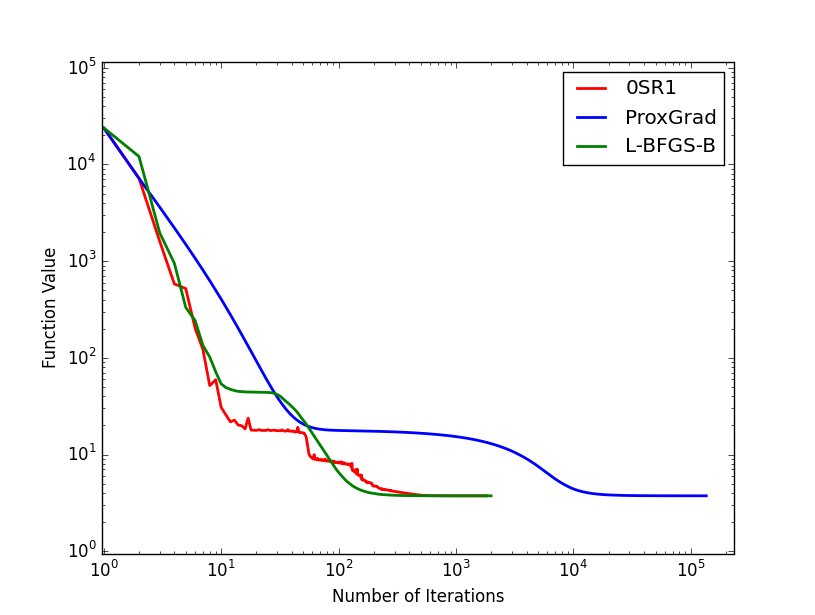
\includegraphics[width = 0.9\textwidth]{ProxNormal_full.png}
\end{frame}
\begin{frame}{Proximal Method}
	\begin{columns}[T]
		\begin{column}{.5\textwidth}
			$F(x) = \lVert Ax - b \rVert + \lambda \lVert x \rVert_1$\\
			$A \in \mathbb{R}^{1500 \times 3000},\:b \in \mathbb{R}^{1500}$\\
			$A_{ij},\:b_i\:$ \textasciitilde $\:\mathcal{N}(0,1)$, $\:\lambda = 0.1$\\
			\vspace{28pt}
			\resizebox{\linewidth}{!}{% This file was created by matplotlib v0.1.0.
% Copyright (c) 2010--2014, Nico Schl�mer <nico.schloemer@gmail.com>
% All rights reserved.
% 
% The lastest updates can be retrieved from
% 
% https://github.com/nschloe/matplotlib2tikz
% 
% where you can also submit bug reports and leavecomments.
% 
\begin{tikzpicture}

\begin{axis}[
xlabel={Number of Iterations},
ylabel={Convergence Factor},
xmin=0, xmax=20,
ymin=0, ymax=1.2,
axis on top,
legend entries={{0SR1},{ProxGrad},{L-BFGS-B}}
]
\addplot [thick, red]
coordinates {
(0,0.848084289429647)
(1,0.571531400706569)
(2,0.3183225225932)
(3,0.325478497212272)
(4,0.229202978836947)
(5,0)

};
\addplot [thick, blue]
coordinates {
(0,0.848084289429647)
(1,0.8761766786044)
(2,0.880353893444499)
(3,0.87631111105461)
(4,0.86750215311503)
(5,0.854873771332014)
(6,0.838545313511358)
(7,0.818309544143084)
(8,0.79368954997227)
(9,0.764405434650521)
(10,0.730785088934228)
(11,0.693056976527169)
(12,0.648410891181648)
(13,0.596467221748105)
(14,0.534977444909731)
(15,0.437803770596474)
(16,0.237479072114323)
(17,0)

};
\addplot [thick, green!50.0!black]
coordinates {
(0,1.03508957652092)
(1,0.953934356298228)
(2,0.781748660719143)
(3,0.348075428829538)
(4,0.392758852840426)
(5,0.321571723894868)
(6,0.494833621279672)
(7,0.62180136584259)
(8,0.66911034267718)
(9,0)

};
\path [draw=black, fill opacity=0] (axis cs:13,0)--(axis cs:13,0);

\path [draw=black, fill opacity=0] (axis cs:13,1)--(axis cs:13,1);

\path [draw=black, fill opacity=0] (axis cs:0,13)--(axis cs:0,13);

\path [draw=black, fill opacity=0] (axis cs:1,13)--(axis cs:1,13);

\end{axis}

\end{tikzpicture}}
		\end{column}\hfill
		\begin{column}{.5\textwidth}
			$F(x) = \lVert Ax - b \rVert + \lambda \lVert x \rVert_1$\\
			$A \in \mathbb{R}^{2197 \times 2197},\:b \in \mathbb{R}^{2197}$\\
			$A$: \small Discretization of 3D Laplacian\\
			\normalsize$\lambda = 1$\\
			\vspace{10pt}
			\resizebox{\linewidth}{!}{% This file was created by matplotlib v0.1.0.
% Copyright (c) 2010--2014, Nico Schl�mer <nico.schloemer@gmail.com>
% All rights reserved.
% 
% The lastest updates can be retrieved from
% 
% https://github.com/nschloe/matplotlib2tikz
% 
% where you can also submit bug reports and leavecomments.
% 
\begin{tikzpicture}

\begin{axis}[
xlabel={Number of Iterations},
ylabel={Convergence Factor},
xmin=0, xmax=20,
ymin=0, ymax=1.2,
axis on top,
legend entries={{0SR1},{ProxGrad},{L-BFGS-B}}
]
\addplot [thick, red]
coordinates {
(0,0.848084289429647)
(1,0.571531400706569)
(2,0.3183225225932)
(3,0.325478497212281)
(4,0.229202978836935)
(5,0)

};
\addplot [thick, blue]
coordinates {
(0,0.848084289429647)
(1,0.8761766786044)
(2,0.880353893444499)
(3,0.87631111105461)
(4,0.86750215311503)
(5,0.854873771332013)
(6,0.838545313511358)
(7,0.818309544143084)
(8,0.79368954997227)
(9,0.764405434650521)
(10,0.730785088934228)
(11,0.693056976527169)
(12,0.648410891181648)
(13,0.596467221748105)
(14,0.534977444909731)
(15,0.437803770596473)
(16,0.237479072114322)
(17,0)

};
\addplot [thick, green!50.0!black]
coordinates {
(0,1.03508957652092)
(1,0.953934356298228)
(2,0.781748660719143)
(3,0.348075428829538)
(4,0.392758852840426)
(5,0.321571723894868)
(6,0.494833621279672)
(7,0.62180136584259)
(8,0.66911034267718)
(9,0)

};
\path [draw=black, fill opacity=0] (axis cs:13,0)--(axis cs:13,0);

\path [draw=black, fill opacity=0] (axis cs:13,1)--(axis cs:13,1);

\path [draw=black, fill opacity=0] (axis cs:0,13)--(axis cs:0,13);

\path [draw=black, fill opacity=0] (axis cs:1,13)--(axis cs:1,13);

\end{axis}

\end{tikzpicture}}
		\end{column}
	\end{columns}
\end{frame}

\begin{frame}{Proximal Method}
	\centering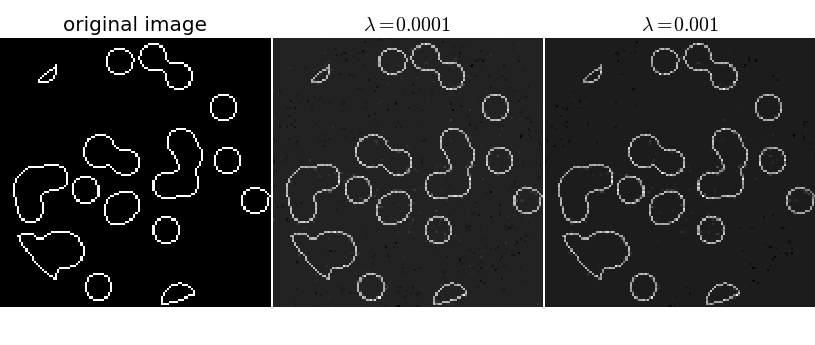
\includegraphics[width=0.9\textwidth]{lambda1.png}\\
	\centering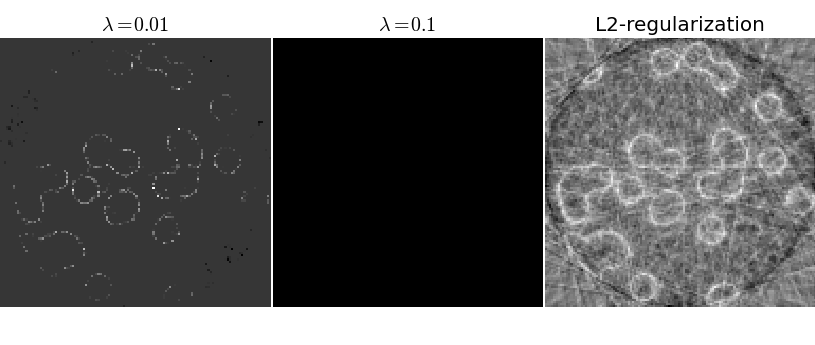
\includegraphics[width=0.9\textwidth]{lambda2.png}

\end{frame}


\begin{frame}
	\begin{figure}[h!]
		\centering
		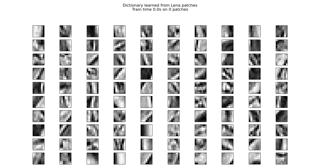
\includegraphics[scale=0.25]{lena_dictionary.png}
		\caption{Dictionary learned}
	\end{figure}
	
\end{frame}
\end{document}

\newpage


\end{document}












